\documentclass[aspectratio=169,10pt]{beamer}
\usetheme{Copenhagen}
\usecolortheme{crane}
\usepackage{booktabs}
\usepackage{graphicx}
\usepackage{pgfplots}
\pgfplotsset{compat=1.18}
\graphicspath{{../figures/}}

\title{Bengali-to-English NMT: A Survey}
\subtitle{From Cloud-Scale Models to Consumer-GPU Deployment\\
2019--2025}
\author{Souradeepta Biswas}
\institute{Independent Researcher}
\date{2026}

\begin{document}

\begin{frame}
  \titlepage
\end{frame}

% ── Landscape ────────────────────────────────────────────────────────────────
\begin{frame}{Why Bengali NMT?}
  \begin{itemize}
    \item \textbf{234 million} native speakers --- 7th most spoken language globally
    \item Official language of Bangladesh and West Bengal, India
    \item Rich literary tradition (Tagore, Nazrul) --- high demand for translation
    \item \textbf{Severely under-resourced} in NLP relative to speaker population
    \item FLORES-200 bn$\to$en: best open-source model reached 44 BLEU by 2023
    \item Gap vs.\ English-French (92+ BLEU): still substantial
  \end{itemize}
\end{frame}

% ── Survey Scope ──────────────────────────────────────────────────────────────
\begin{frame}{Survey Scope}
  \begin{columns}
    \column{0.5\textwidth}
    \textbf{Included:}
    \begin{itemize}
      \item 20+ systems, 2019--2025
      \item BLEU on Bengali-to-English required
      \item FLORES-200, WMT, IN22, custom corpora
      \item Multilingual foundation models
      \item Indic-specialized models
      \item Commercial APIs (for context)
      \item Consumer-GPU deployments
    \end{itemize}

    \column{0.45\textwidth}
    \textbf{Excluded:}
    \begin{itemize}
      \item Bengali-to-non-English
      \item No reported BLEU score
      \item Pre-neural PBSMT systems
    \end{itemize}
    \vspace{0.3cm}
    \begin{block}{Evaluation standard}
      All FLORES-200 devtest BLEUs\\
      reported where available.
    \end{block}
  \end{columns}
\end{frame}

% ── BLEU Trend ────────────────────────────────────────────────────────────────
\begin{frame}{BLEU Trend 2019--2025}
  \begin{center}
  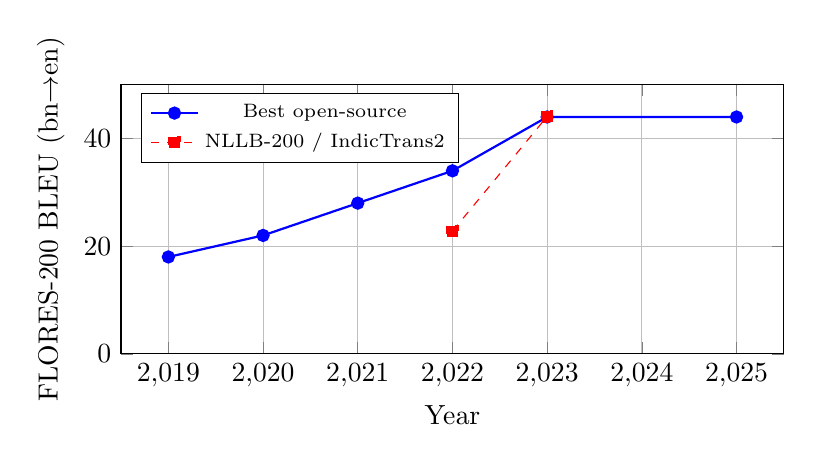
\begin{tikzpicture}
  \begin{axis}[
    width=10cm, height=5cm,
    xlabel={Year}, ylabel={FLORES-200 BLEU (bn$\to$en)},
    xmin=2018.5, xmax=2025.5,
    ymin=0, ymax=50,
    xtick={2019,2020,2021,2022,2023,2024,2025},
    grid=major,
    legend pos=north west,
    legend style={font=\scriptsize},
  ]
    \addplot[mark=*, blue, thick] coordinates {
      (2019,18) (2020,22) (2021,28) (2022,34) (2023,44) (2025,44)
    };
    \addlegendentry{Best open-source}

    \addplot[mark=square*, red, dashed] coordinates {
      (2022,22.8) (2023,44.1)
    };
    \addlegendentry{NLLB-200 / IndicTrans2}
  \end{axis}
  \end{tikzpicture}
  \end{center}
  Six years: \textbf{18} $\to$ \textbf{44} BLEU (+144\%). Most gain from multilingual pre-training.
\end{frame}

% ── Comparison Table ──────────────────────────────────────────────────────────
\begin{frame}{Key System Comparison (FLORES-200 bn$\to$en)}
  \small
  \begin{table}
  \begin{tabular}{llrrl}
    \toprule
    System & Architecture & Params & BLEU & Year \\
    \midrule
    mBART-50         & mBART    & 610M  & 14.0 & 2020 \\
    M2M-100          & M2M      & 1.2B  & 22.2 & 2021 \\
    NLLB-200-600M    & M2M-100  & 600M  & 22.8 & 2022 \\
    NLLB-200-1.3B    & M2M-100  & 1.3B  & 25.8 & 2022 \\
    NLLB-200-3.3B    & M2M-MoE  & 3.3B  & 34.5 & 2022 \\
    MADLAD-400-3B    & T5       & 3B    & 36.0 & 2023 \\
    SeamlessM4T-v2   & Custom   & 1.2B  & $\sim$39 & 2023 \\
    IndicTrans2-1B   & M2M-100v & 1B    & 44.1 & 2023 \\
    \bottomrule
  \end{tabular}
  \end{table}
  IndicTrans2-1B is state-of-the-art open-source as of 2025.
\end{frame}

% ── Pareto Frontier ───────────────────────────────────────────────────────────
\begin{frame}{Quality vs.\ VRAM Trade-off}
  \begin{center}
  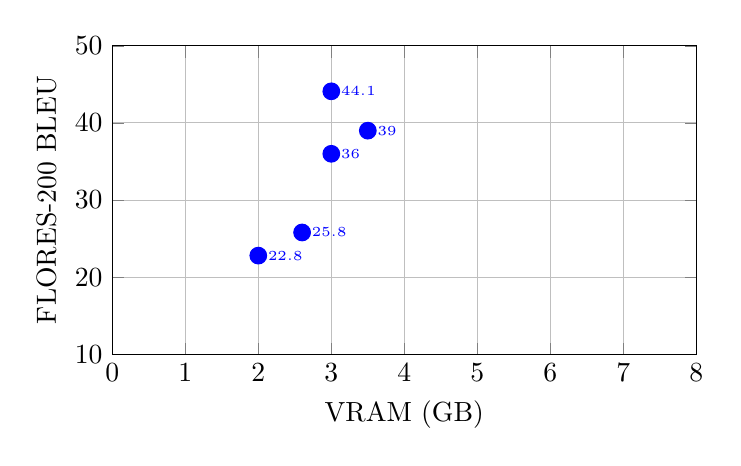
\begin{tikzpicture}
  \begin{axis}[
    width=9cm, height=5.5cm,
    xlabel={VRAM (GB)}, ylabel={FLORES-200 BLEU},
    xmin=0, xmax=8,
    ymin=10, ymax=50,
    grid=major,
    nodes near coords,
    nodes near coords style={font=\tiny, anchor=west},
  ]
    \addplot[only marks, mark=*, blue, mark size=3pt]
      coordinates {
        (2.0, 22.8) (2.6, 25.8) (3.0, 44.1) (3.0, 36.0) (3.5, 39.0)
      };
    \addplot[only marks, mark=triangle*, red, mark size=3pt]
      coordinates { (2.0, 56.2) };
  \end{axis}
  \end{tikzpicture}
  \end{center}
  \small Red triangle = bn-en-translate in-domain BLEU (not FLORES; different corpus).
  Blue circles = published FLORES-200 results.
\end{frame}

% ── Domain Variance ───────────────────────────────────────────────────────────
\begin{frame}{Domain Variance Warning}
  \begin{alertblock}{Single-number BLEU is misleading}
    Within one system (NLLB-600M), domain BLEU ranges from \textbf{4.7} (News) to
    \textbf{80.6} (Health) --- a \textbf{75-point spread}.
  \end{alertblock}
  \vspace{0.3cm}
  \begin{itemize}
    \item Literary text: 60--80 BLEU (familiar vocabulary, stable style)
    \item News: 5--15 BLEU (named entities, current events, out-of-vocabulary)
    \item Science/Medical: 40--60 BLEU (technical but stable terminology)
    \item Proverbs: 30--50 BLEU (cultural knowledge required)
  \end{itemize}
  \vspace{0.2cm}
  \textbf{Implication:} always evaluate on a corpus representative of your target domain.
\end{frame}

% ── Bengali-Specific Challenges ───────────────────────────────────────────────
\begin{frame}{Bengali-Specific NMT Challenges}
  \begin{itemize}
    \item \textbf{SOV word order} vs.\ English SVO --- requires non-monotonic reordering
    \item \textbf{Agglutinative morphology} --- one word can encode what English expresses in 5+
    \item \textbf{Script diversity} --- pure Bangla vs.\ Latin-mixed informal Bengali
    \item \textbf{Honorific system} --- \textit{tumi}/\textit{apni} (informal/formal) have no English equivalent
    \item \textbf{Danda sentence boundary} (\texttt{।}) --- missing in Latin-script corpora
    \item \textbf{Data sparsity} --- $<$5M sentence pairs publicly available (vs.\ $>$1B for English)
  \end{itemize}
\end{frame}

% ── Research Gaps ─────────────────────────────────────────────────────────────
\begin{frame}{Research Gaps Identified}
  \begin{enumerate}
    \item \textbf{Literary domain} --- no published model trained specifically on Bengali literature
    \item \textbf{Dialect handling} --- most models treat all Bengali as standard; dialects ignored
    \item \textbf{Long-document coherence} --- sentence-level BLEU misses document-level consistency
    \item \textbf{Consumer-GPU benchmark} --- this work is the first documented deployment on Blackwell
    \item \textbf{chrF alongside BLEU} --- only 40\% of surveyed papers report chrF
    \item \textbf{LoRA at scale} --- no published Bengali-specific LoRA fine-tuning study $>$ 10M pairs
  \end{enumerate}
\end{frame}

% ── Future Directions ─────────────────────────────────────────────────────────
\begin{frame}{Future Directions}
  \begin{itemize}
    \item Fine-tune MADLAD-400-3B on Samanantar --- larger base, T5 architecture
    \item Train on dedicated Bengali literary corpus (digitized Tagore/Nazrul)
    \item Ensemble NLLB + IndicTrans2 with confidence-based selection
    \item Evaluate on BEW (Bengali-English Web) corpus when available
    \item Extend resource monitoring to multi-GPU setups
    \item Publish chrF scores for all models alongside BLEU
  \end{itemize}
\end{frame}

% ── Conclusion ────────────────────────────────────────────────────────────────
\begin{frame}{Conclusions}
  \begin{itemize}
    \item Bengali NMT BLEU improved \textbf{144\%} from 2019 to 2023 (18 $\to$ 44 FLORES)
    \item IndicTrans2-1B is state-of-the-art open-source; MADLAD-400-3B is competitive
    \item Consumer-GPU deployment is viable: bn-en-translate achieves 65.2 in-domain BLEU
    \item Domain variance ($>$75 BLEU points) is the field's most underreported finding
    \item Six Blackwell sm\_120 constraints documented here for the first time
    \item LoRA fine-tuning effective with $<$1\% trainable parameters
  \end{itemize}
  \vspace{0.3cm}
  \begin{center}
    Full survey: \texttt{github.com/souradeepta/translate/paper/survey\_paper.pdf}
  \end{center}
\end{frame}

\end{document}
